%%%%%%%%%%%%%%%%%%%%%%%%%%%%%%%%%%%%%%%%%
% Beamer Presentation
% LaTeX Template
% Version 1.0 (10/11/12)
%
% This template has been downloaded from:
% http://www.LaTeXTemplates.com
%
% License:
% CC BY-NC-SA 3.0 (http://creativecommons.org/licenses/by-nc-sa/3.0/)
%
%%%%%%%%%%%%%%%%%%%%%%%%%%%%%%%%%%%%%%%%%

%----------------------------------------------------------------------------------------
% PACKAGES AND THEMES
%----------------------------------------------------------------------------------------

\documentclass[12pt,xcolor={dvipsnames}]{beamer}
%\setbeamersize{text margin left=1em,text margin right=1em}
\usepackage{mathtools}
\usepackage{amsmath}
\usepackage{bm}
\usepackage{hyperref}

\usepackage{graphicx} % Allows including images
\graphicspath{{/Users/rebecca/Documents/JER/MinimiseMatrixJER/MCvsData_PowhegPythia/}{/Users/rebecca/Documents/JER/MinimiseMatrixJER/}{/Users/rebecca/Documents/JER/MinimiseMatrixJER/PowhegPythiavsSherpa/}{/Users/rebecca/Documents/Presentations/Talks/}}
\usepackage{booktabs} % Allows the use of \toprule, \midrule and \bottomrule in tables

\usepackage{etoolbox}

\usepackage{subcaption}
\captionsetup{compatibility=false}

\usepackage{multirow}

\usepackage{appendixnumberbeamer}

%\newlength\origleftmargini
%\setlength\origleftmargini\leftmargini
%\setbeamertemplate{itemize/enumerate body begin}{\setlength{\leftmargini}{2pt}}%

%\let\oldexampleblock\exampleblock
%\let\oldendexampleblock\endexampleblock
%\def\exampleblock{\begingroup \setbeamertemplate{itemize/enumerate body begin}{\setlength{\leftmargini}{\origleftmargini}} \oldexampleblock}
%\def\endexampleblock{\oldendexampleblock \endgroup}%

%\let\oldalertblock\alertblock
%\let\oldendalertblock\endalertblock
%\def\alertblock{\begingroup \setbeamertemplate{itemize/enumerate body begin}{\setlength{\leftmargini}{\origleftmargini}} \oldalertblock}
%\def\endalertblock{\oldendalertblock \endgroup}

\mode<presentation> {

% The Beamer class comes with a number of default slide themes
% which change the colors and layouts of slides. Below this is a list
% of all the themes, uncomment each in turn to see what they look like.

%\usetheme{default}
%\usetheme{AnnArbor}
%\usetheme{Antibes}
%\usetheme{Bergen}
%\usetheme{Berkeley}
%\usetheme{Berlin}
\usetheme{Boadilla}
%\usetheme{CambridgeUS}
%\usetheme{Copenhagen}
%\usetheme{Darmstadt}
%\usetheme{Dresden}
%\usetheme{Frankfurt}
%\usetheme{Goettingen}
%\usetheme{Hannover}
%\usetheme{Ilmenau}
%\usetheme{JuanLesPins}
%\usetheme{Luebeck}
%\usetheme{Madrid}
%\usetheme{Malmoe}
%\usetheme{Marburg}
%\usetheme{Montpellier}
%\usetheme{PaloAlto}
%\usetheme{Pittsburgh}
%\usetheme{Rochester}
%\usetheme{Seahorse}
%\usetheme{Singapore}
%\usetheme{Szeged}
%\usetheme{Warsaw}

% As well as themes, the Beamer class has a number of color themes
% for any slide theme. Uncomment each of these in turn to see how it
% changes the colors of your current slide theme.

%\usecolortheme{albatross}
%\usecolortheme{beaver}
%\usecolortheme{beetle}
%\usecolortheme{crane}
%\usecolortheme{dolphin}
%\usecolortheme{dove}
%\usecolortheme{fly}
%\usecolortheme{lily}
%\usecolortheme{RoyalBlue}
%\usecolortheme{rose}
%\usecolortheme{seagull}
%\usecolortheme{seahorse}
%\usecolortheme{whale}
%\usecolortheme{wolverine}

%%Changing the theme colours
%\setbeamercolor*{structure}{bg=Plum!20,fg=Plum}
%\setbeamercolor*{palette primary}{use=structure,fg=white,bg=structure.fg}
%\setbeamercolor*{palette secondary}{use=structure,fg=white,bg=structure.fg!75}
%\setbeamercolor*{palette tertiary}{use=structure,fg=white,bg=structure.fg!50!black}
%\setbeamercolor*{palette quaternary}{fg=white,bg=black}
%\setbeamercolor{section in toc}{fg=black,bg=white}
%%\setbeamercolor{alerted text}{use=structure,fg=structure.fg!50!black!80!black}
%\setbeamercolor{titlelike}{parent=palette primary,fg=structure.fg!50!black}
%\setbeamercolor{frametitle}{bg=gray!30!white,fg=Plum}
%\setbeamercolor*{titlelike}{parent=palette primary}

%Changing the theme colours
\setbeamercolor*{structure}{bg=RoyalPurple,fg=RoyalPurple}
\setbeamercolor*{palette primary}{use=structure,fg=white,bg=structure.fg}
\setbeamercolor*{palette secondary}{use=structure,fg=white,bg=structure.fg}
\setbeamercolor*{palette tertiary}{use=structure,fg=white,bg=structure.fg}
\setbeamercolor*{palette quaternary}{fg=white,bg=black}
\setbeamercolor{section in toc}{fg=black,bg=white}
%\setbeamercolor{alerted text}{use=structure,fg=structure.fg!50!black!80!black}
\setbeamercolor{titlelike}{parent=palette primary,fg=structure.fg!50!black}
%\setbeamercolor{frametitle}{use=structure,fg=white,bg=structure.fg}
\setbeamercolor*{titlelike}{parent=palette primary}

%\setbeamercolor{block}{bg=yellow!10,fg=black}
%\setbeamercolor{block title}{bg=yellow!50,fg=black}
%\AtBeginEnvironment{block}{\setbeamercolor{itemize item}{fg=yellow}}

\newenvironment<>{examplefirst}[1]{%
  \setbeamercolor{block title}{bg=yellow!50,fg=black}%
  \begin{block}#2{#1}}{\end{block}}
\AtBeginEnvironment{examplefirst}{\setbeamercolor{itemize item}{fg=yellow}}

%\setbeamertemplate{footline} % To remove the footer line in all slides uncomment this line
%\setbeamertemplate{footline}[page number] % To replace the footer line in all slides with a simple slide count uncomment this line

%\setbeamertemplate{navigation symbols}{} % To remove the navigation symbols from the bottom of all slides uncomment this line


\setbeamertemplate{blocks}[rounded][shadow=false]
\setbeamertemplate{itemize items}[circle]
\setbeamertemplate{itemize subitems}[circle]

\renewcommand{\thefootnote}{\alph{footnote}}

}

%----------------------------------------------------------------------------------------
% TITLE PAGE
%----------------------------------------------------------------------------------------



\title[Jet Energy Resolution Plots]{Jet Energy Resolution for the Dijet Balance Method} % The short title appears at the bottom of every slide, the full title is only on the title page

\author{\underline{Rebecca Pickles}, Darren Price} % Your name
%\institute[UoM] % Your institution as it will appear on the bottom of every slide, may be shorthand to save space
%{
%University of Manchester\\ % Your institution for the title page
%\medskip
%\textit{julia.iturbe@cern.ch} % Your email address
%}
% logo of my university
\titlegraphic{
\includegraphics[width=3cm]{UniOfManchesterLogo}}
\date{\today} % Date, can be changed to a custom date

\begin{document}


\begin{frame}
\titlepage % Print the title page as the first slide
\end{frame}

\iffalse
\begin{frame}
\frametitle{Overview} % Table of contents slide, comment this block out to remove it
\tableofcontents % Throughout your presentation, if you choose to use \section{} and \subsection{} commands, these will automatically be printed on this slide as an overview of your presentation
\end{frame}
\fi
%----------------------------------------------------------------------------------------
% PRESENTATION SLIDES
%----------------------------------------------------------------------------------------

%------------------------------------------------
\section{Introduction} % Sections can be created in order to organize your presentation into discrete blocks, all sections and subsections are automatically printed in the table of contents as an overview of the talk

%------------------------------------------------
\iffalse

\fi

\begin{frame}
\frametitle{Status}
\begin{itemize}
\item Started looking at the fits for the 25GeV $<$ pTavg $<$ 40GeV.
\item Started to look at subtracting the MC Truth resolution from the MC Reco and Data for Sherpa
\item Compared Powheg+Pythia8 with Sherpa for EM+JES and Truth
\item Corrected resolution calculation due to the EtaInterCalibration method's deviation from the original method of calculating Asymmetry ( factor of $\sqrt{2}$ ) 
\end{itemize}
\end{frame}

\begin{frame}
\frametitle{JER vs Eta: 25 $<$ pTavg $<$ 40}
\center{\includegraphics[width=8cm, height=6cm]{25pTavg40_MCvsData.pdf}}
\begin{itemize}
\item Truth MC has a higher resolution than Reco MC. 
\end{itemize}
\end{frame}

\begin{frame}
\frametitle{JER vs Eta: 25 $<$ pTavg $<$ 40 : Data fits}
\center{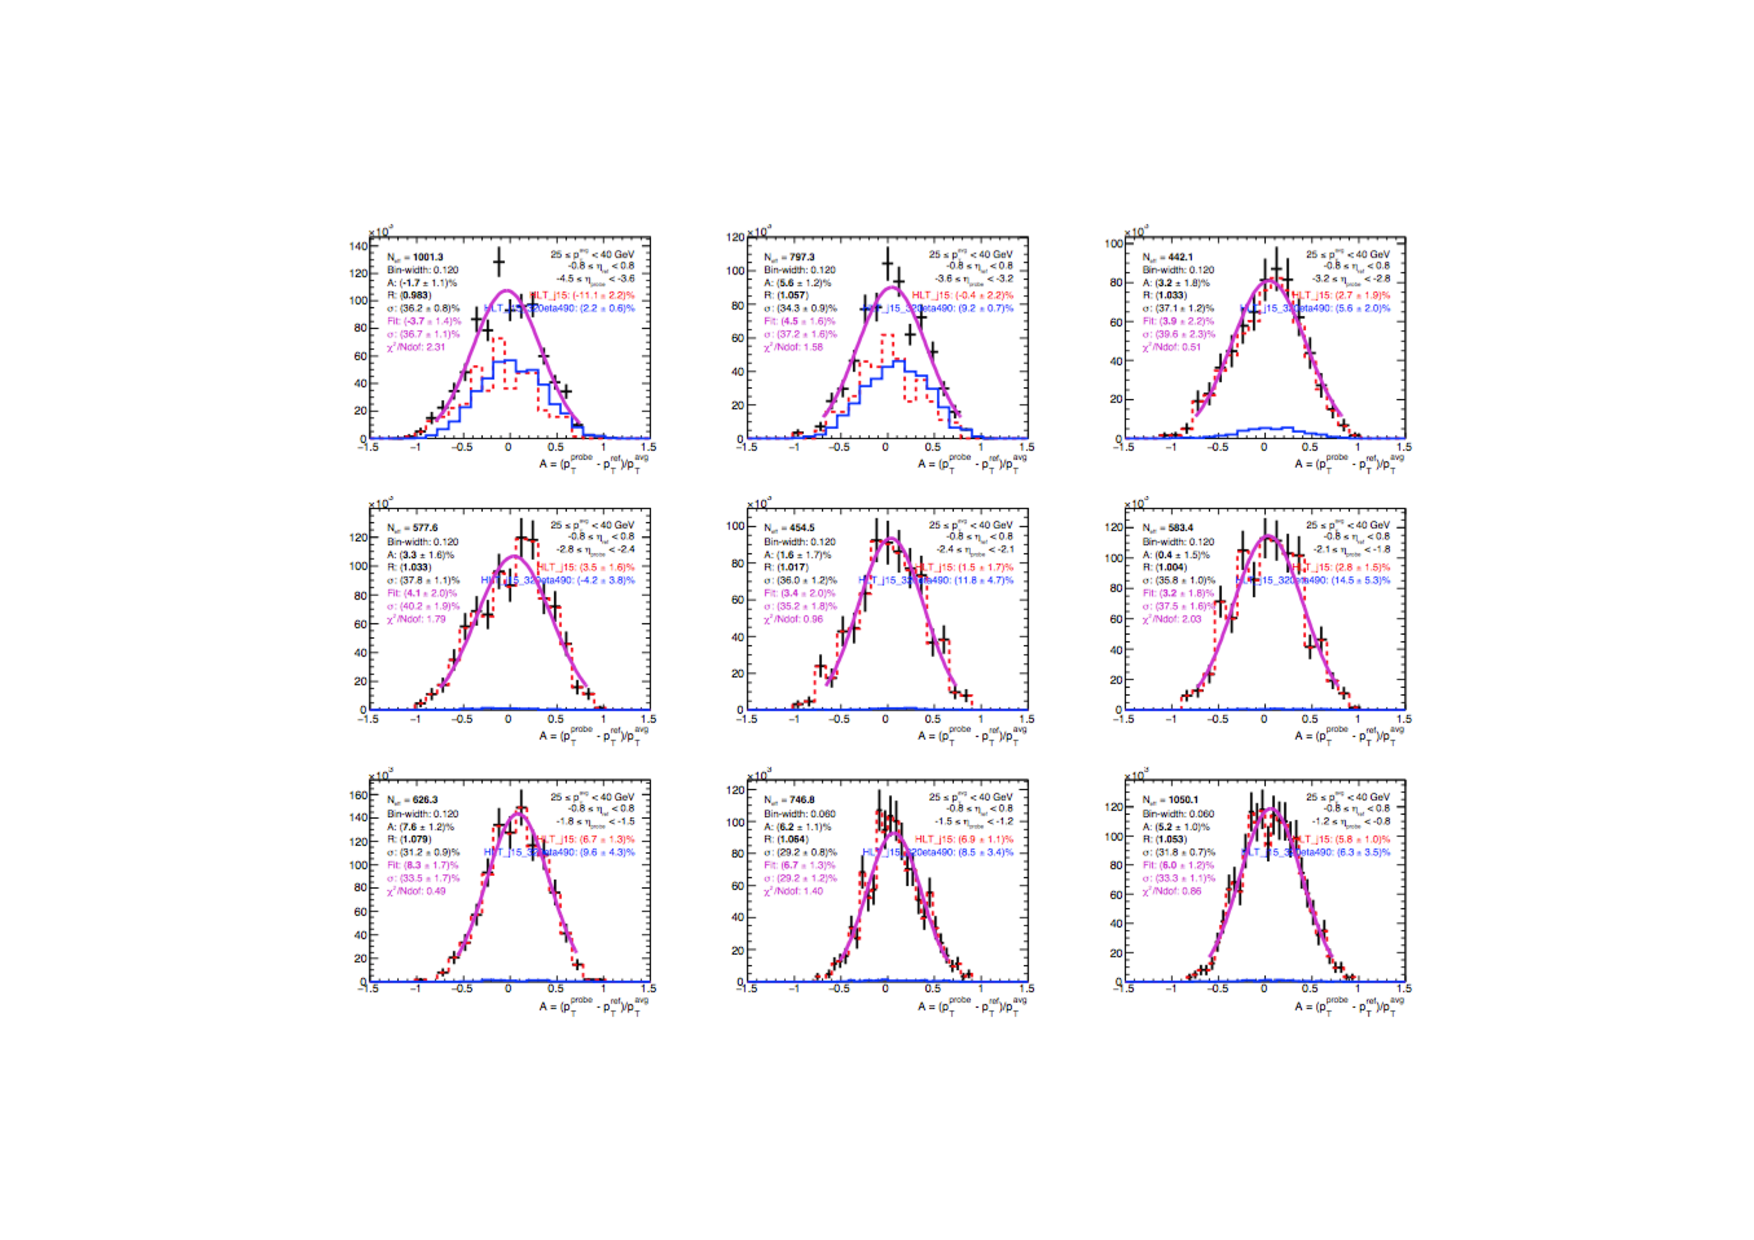
\includegraphics[width=9cm, height=6.5cm]{25to40DataFits1.pdf}}
\end{frame}

\begin{frame}
\frametitle{JER vs Eta: 25 $<$ pTavg $<$ 40 : Data fits}
\center{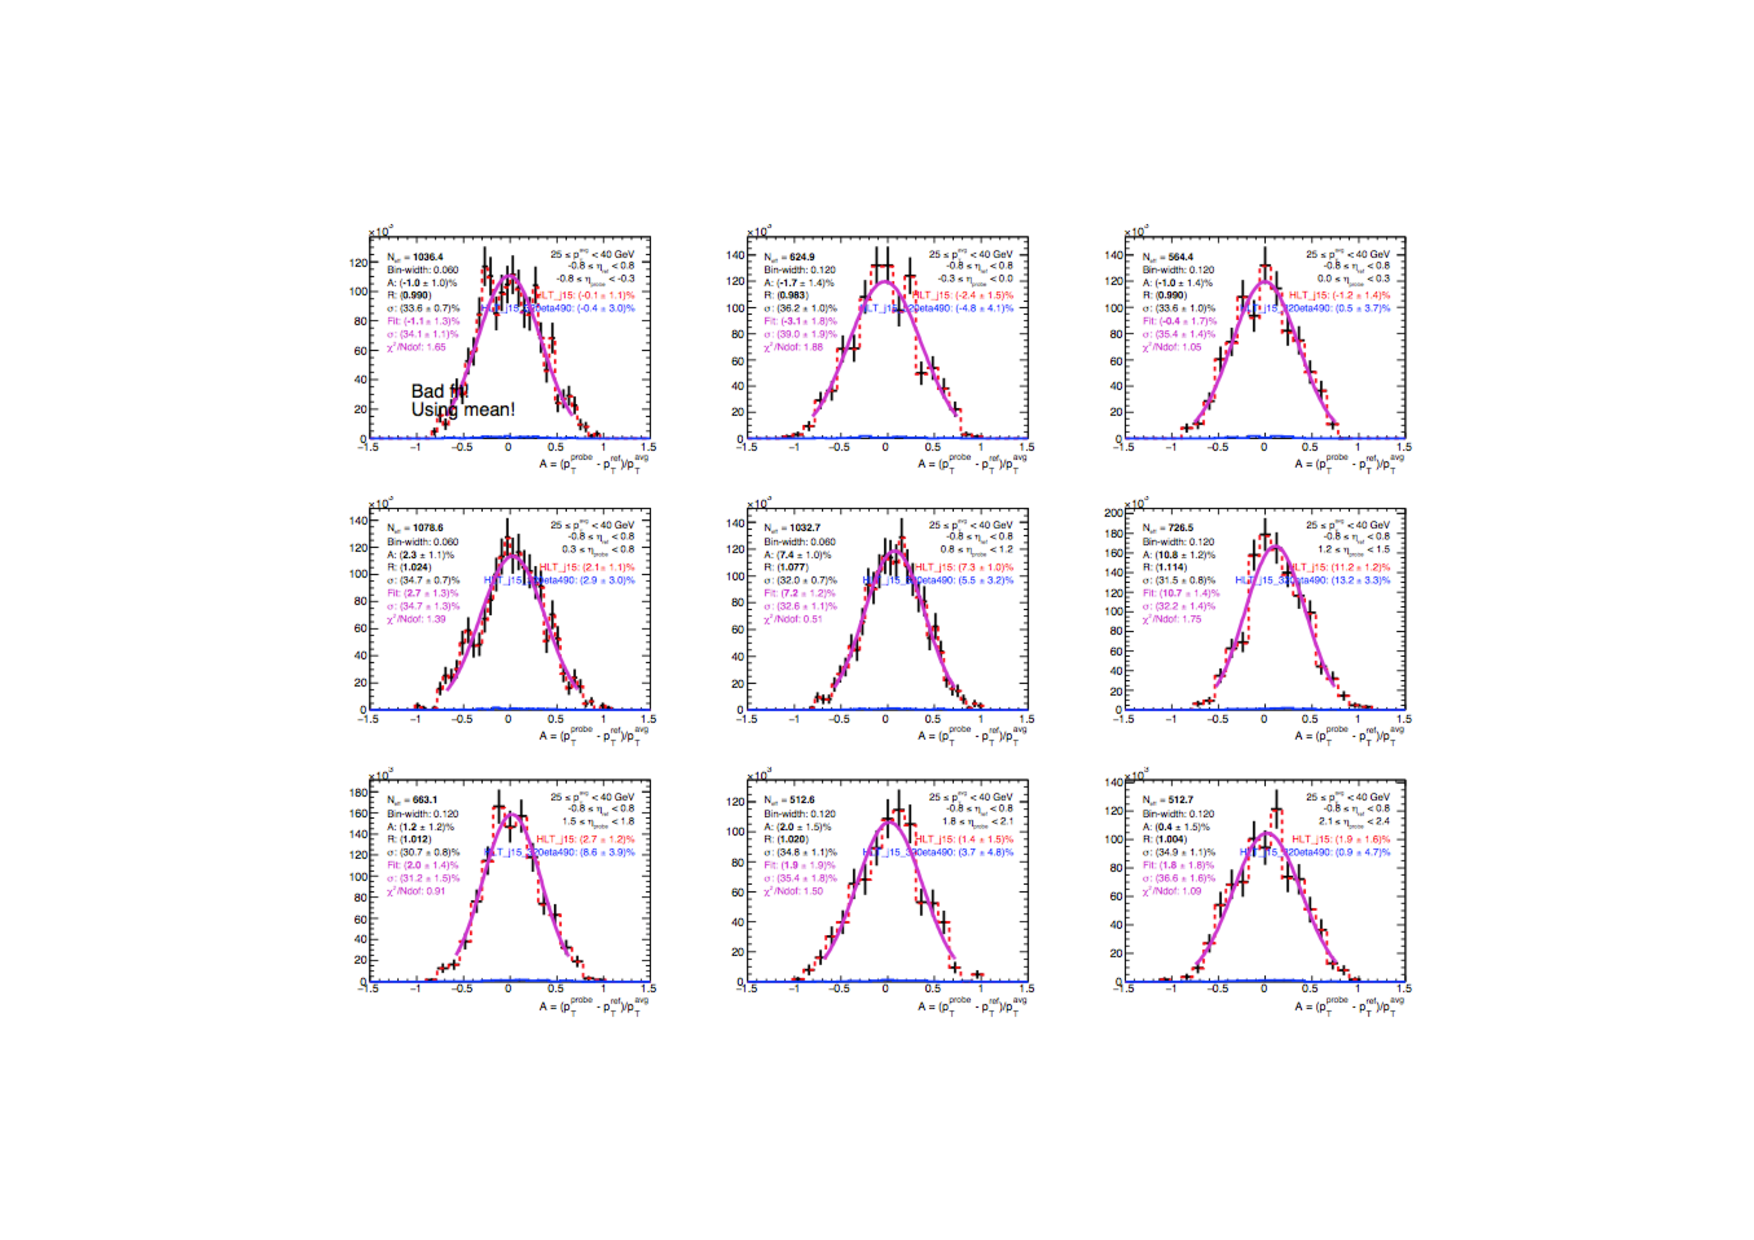
\includegraphics[width=9cm, height=6.5cm]{25to40DataFits2.pdf}}
\end{frame}

\begin{frame}
\frametitle{JER vs Eta: 25 $<$ pTavg $<$ 40 : Data fits}
\center{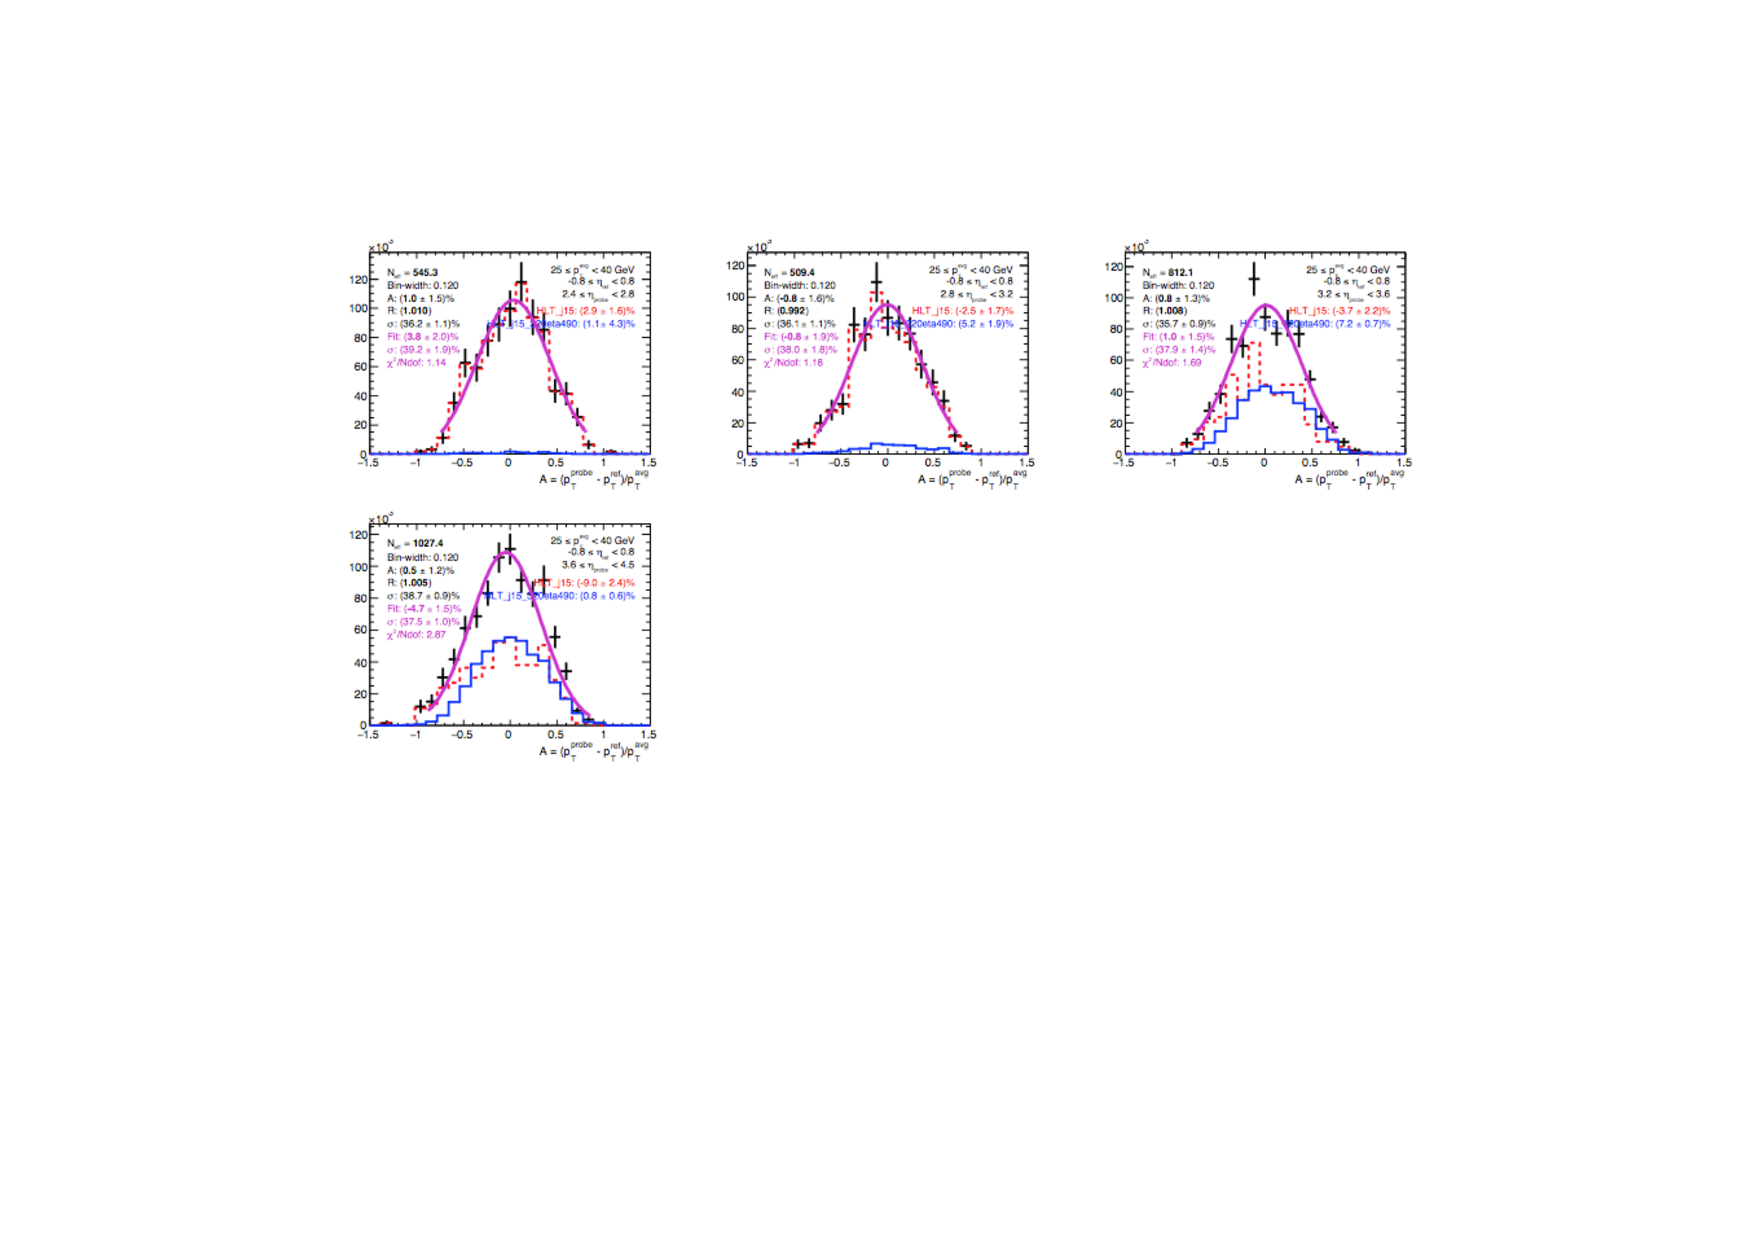
\includegraphics[width=9cm, height=5cm]{25to40DataFits3.pdf}}
\end{frame}


\begin{frame}
\frametitle{JER vs Eta: 25 $<$ pTavg $<$ 40 : Powheg+Pythia8 EM+JES fits}
\center{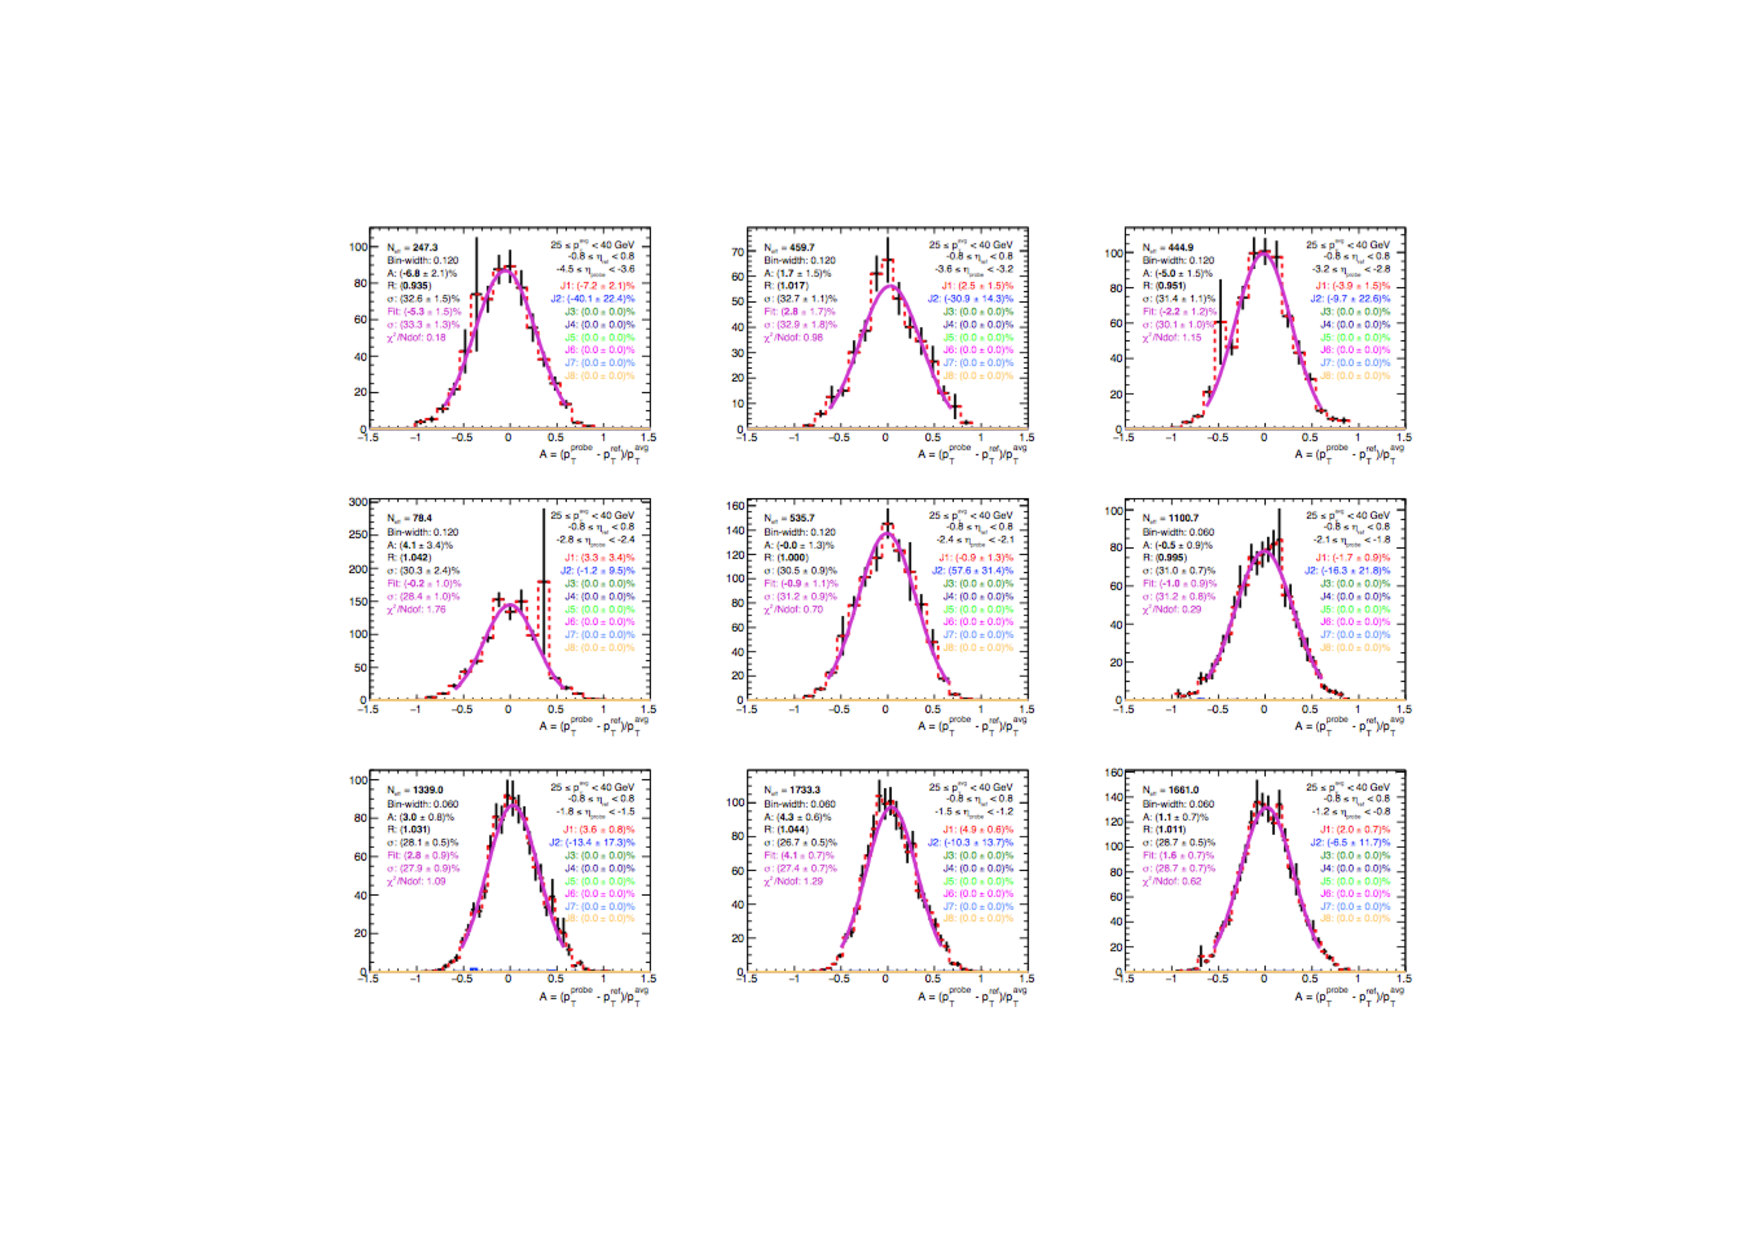
\includegraphics[width=9cm, height=6.5cm]{25to40PPEMJESFits1.pdf}}
\end{frame}

\begin{frame}
\frametitle{JER vs Eta: 25 $<$ pTavg $<$ 40 : Powheg+Pythia8 EM+JES fits}
\center{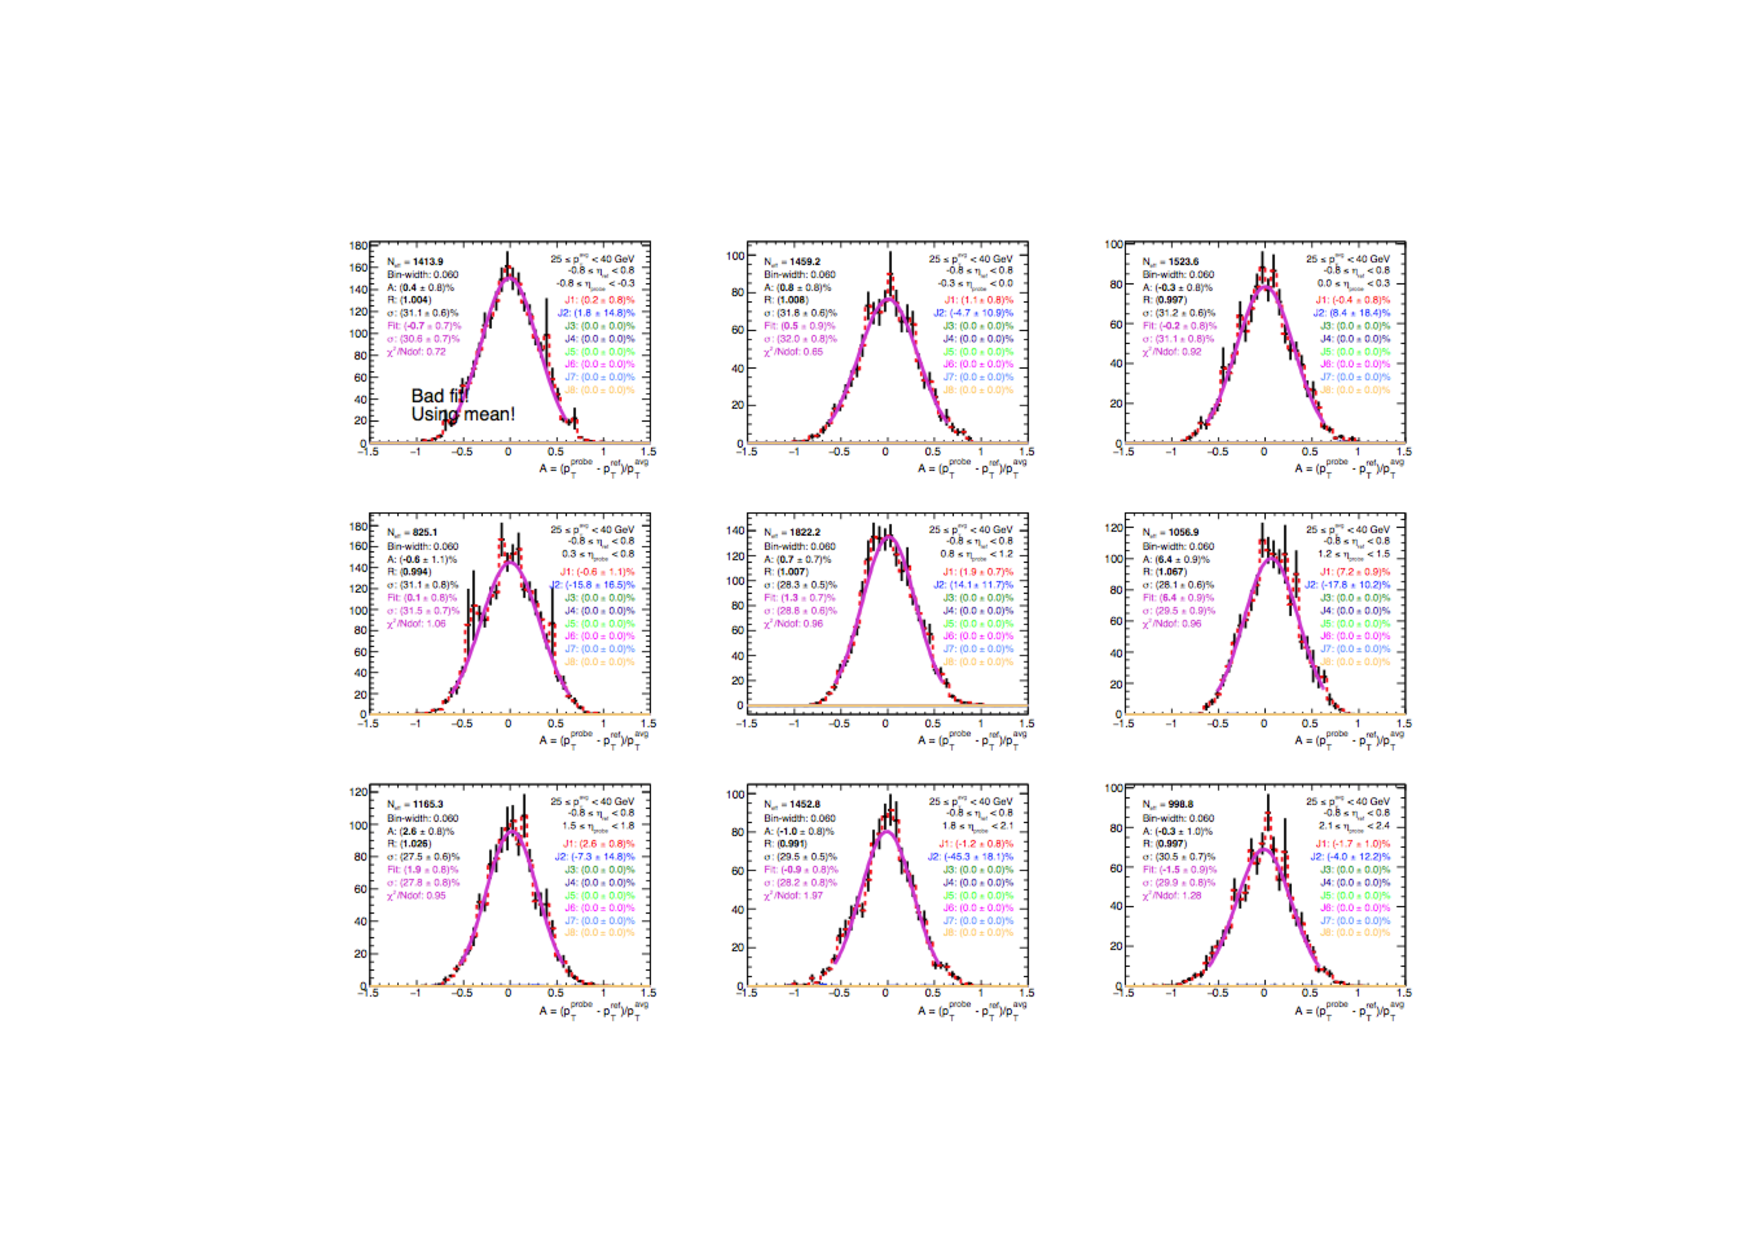
\includegraphics[width=9cm, height=6.5cm]{25to40PPEMJESFits2.pdf}}
\end{frame}

\begin{frame}
\frametitle{JER vs Eta: 25 $<$ pTavg $<$ 40 : Powheg+Pythia8 EM+JES fits}
\center{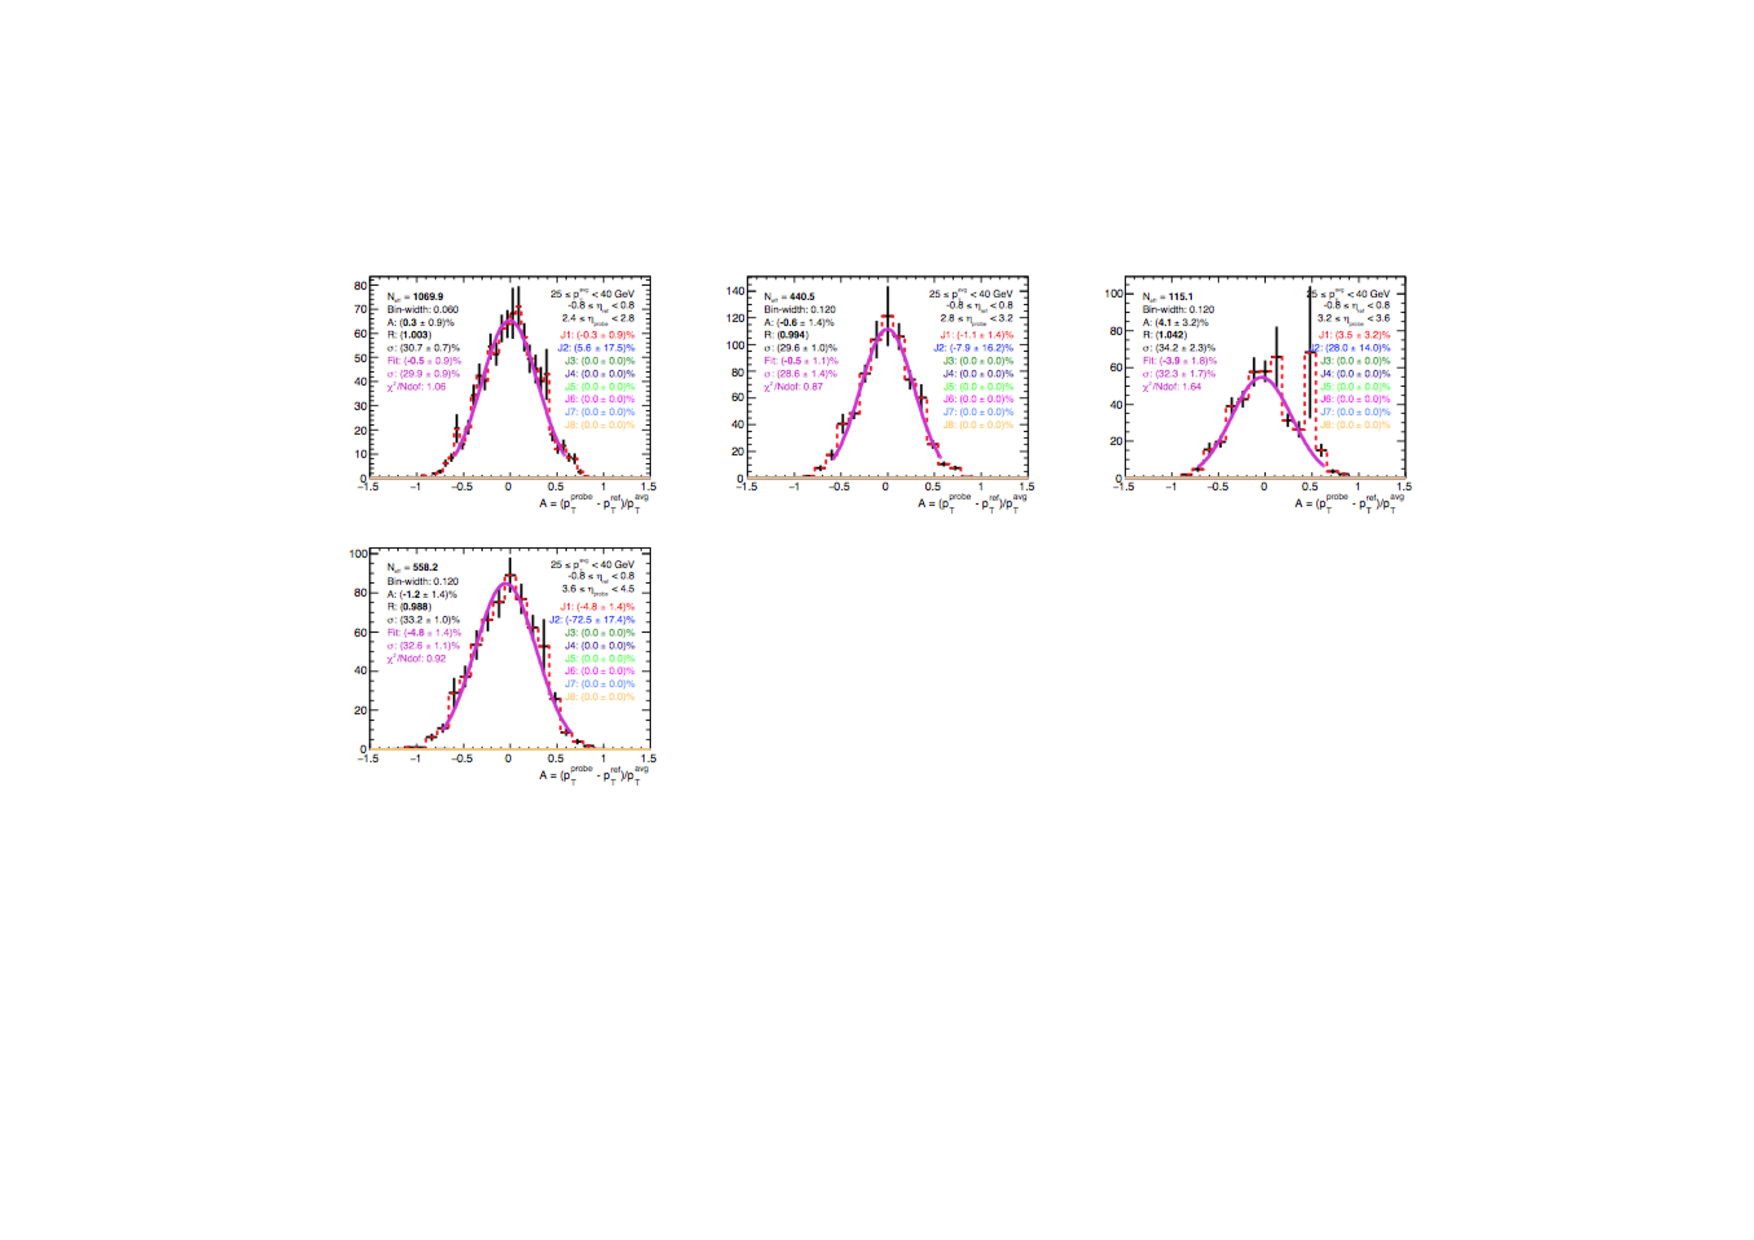
\includegraphics[width=9cm, height=5cm]{25to40PPEMJESFits3.pdf}}
\end{frame}

\begin{frame}
\frametitle{JER vs Eta: 25 $<$ pTavg $<$ 40 : Powheg+Pythia8 Truth fits}
\center{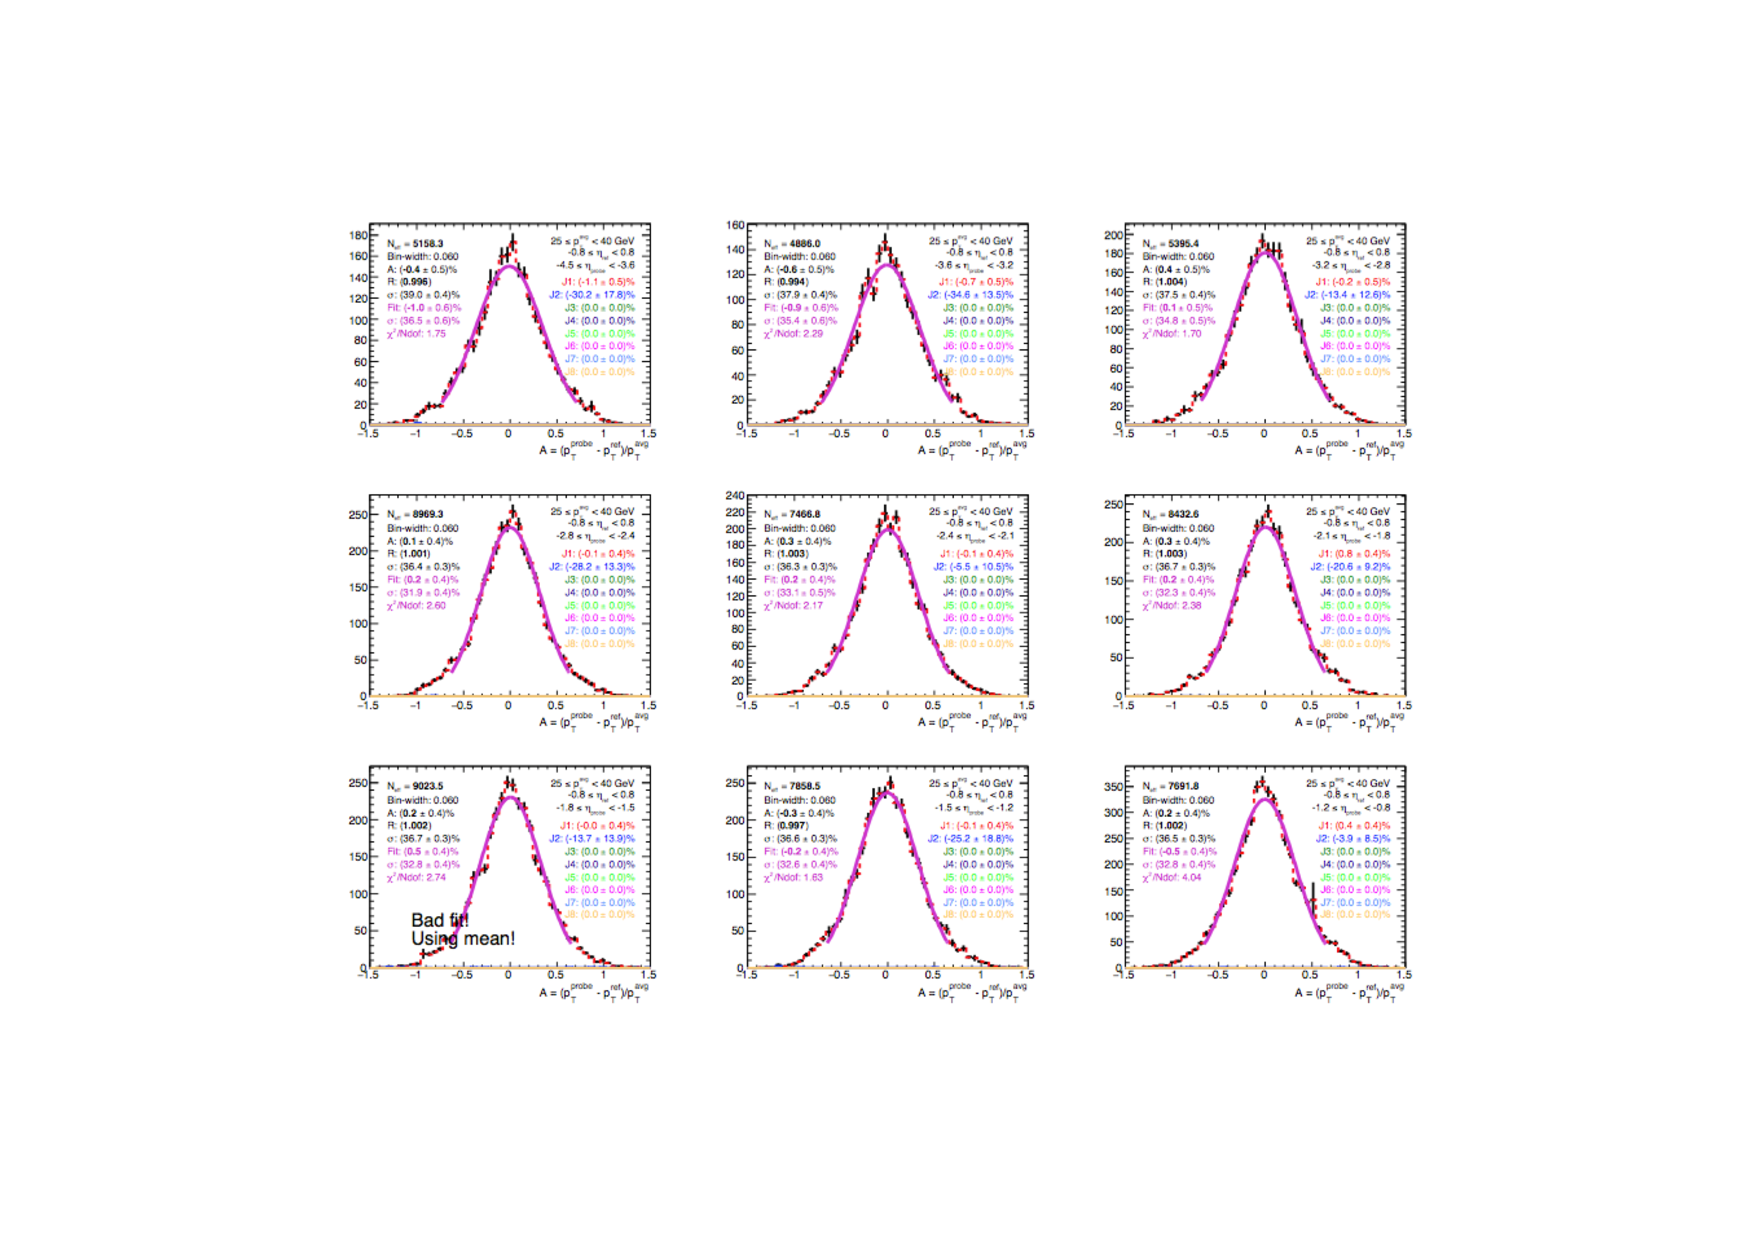
\includegraphics[width=9cm, height=6.5cm]{25to40PPTruthFits1.pdf}}
\end{frame}

\begin{frame}
\frametitle{JER vs Eta: 25 $<$ pTavg $<$ 40 : Powheg+Pythia8 Truth fits}
\center{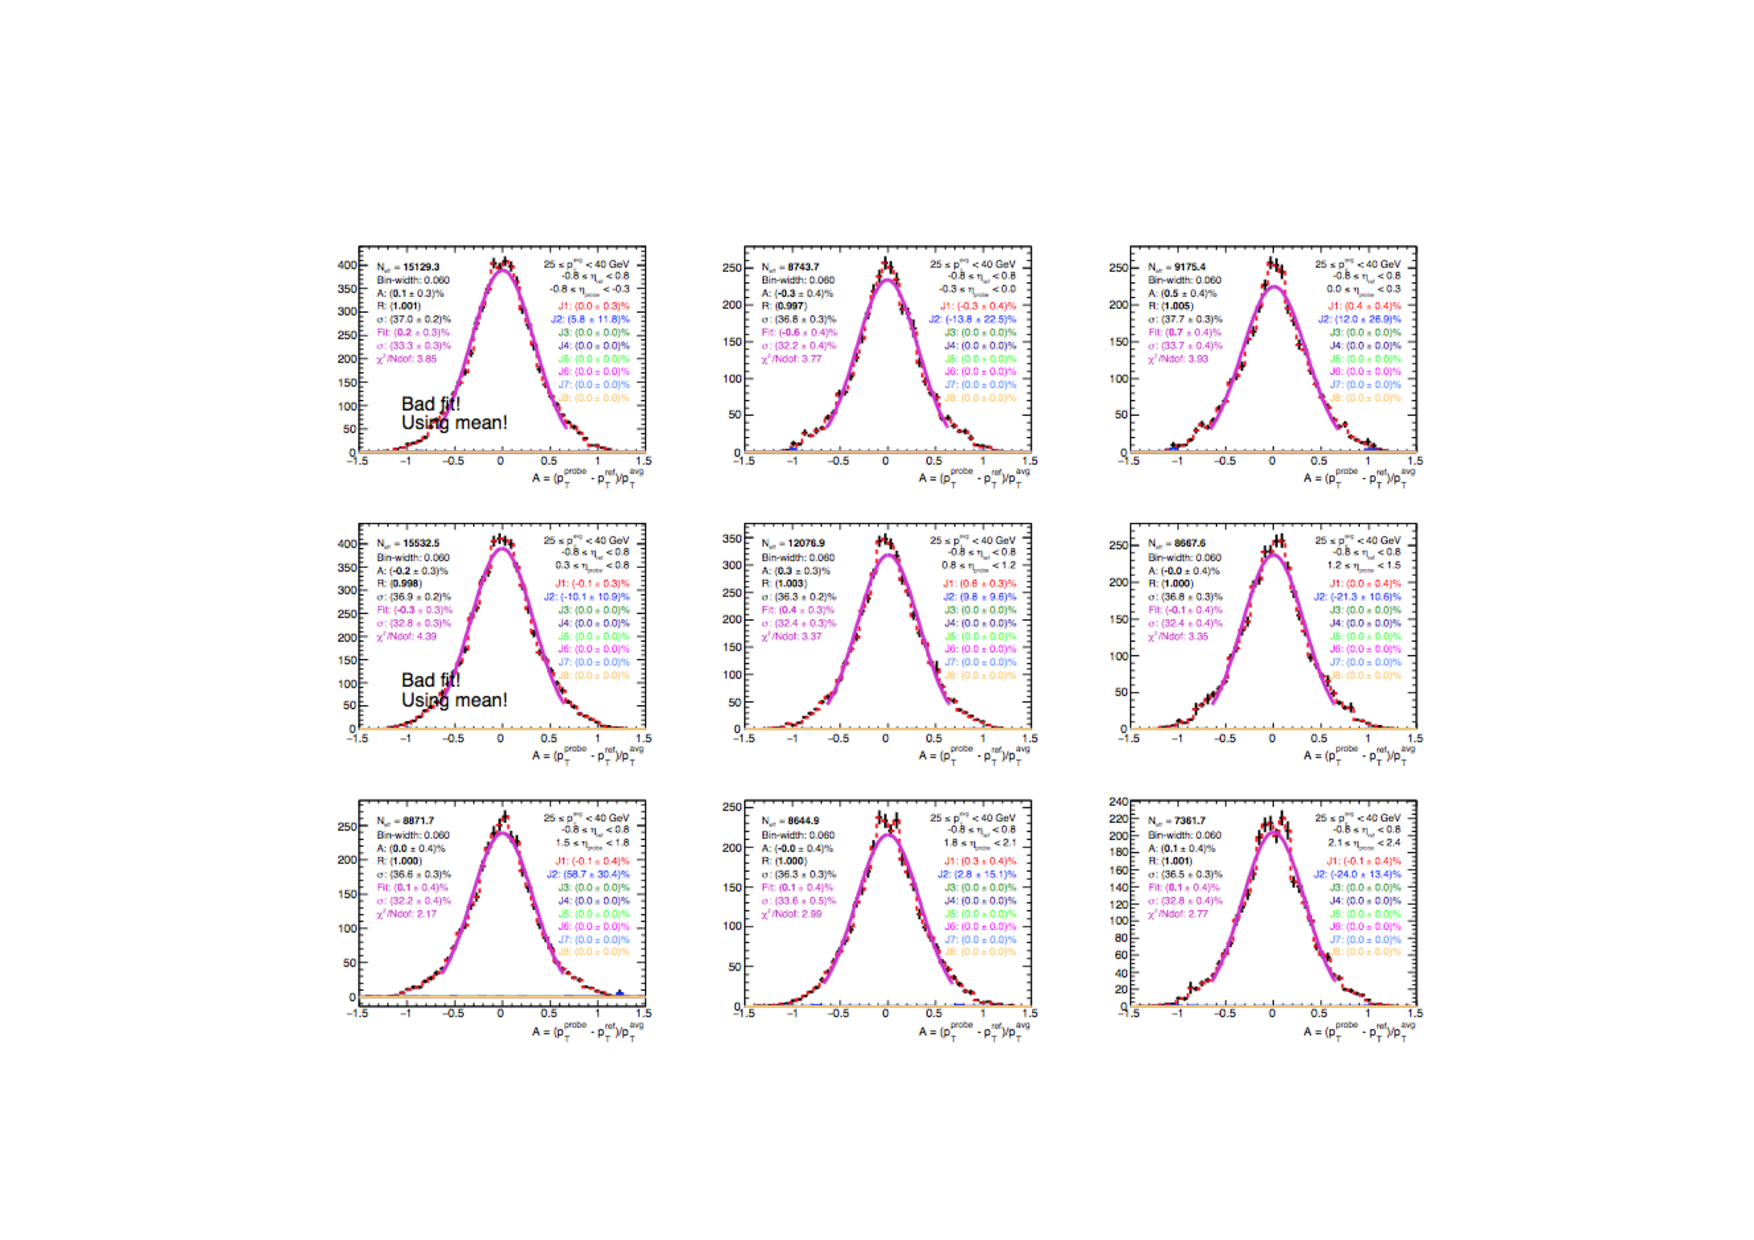
\includegraphics[width=9cm, height=6.5cm]{25to40PPTruthFits2.pdf}}
\end{frame}

\begin{frame}
\frametitle{JER vs Eta: 25 $<$ pTavg $<$ 40 : Powheg+Pythia8 Truth fits}
\center{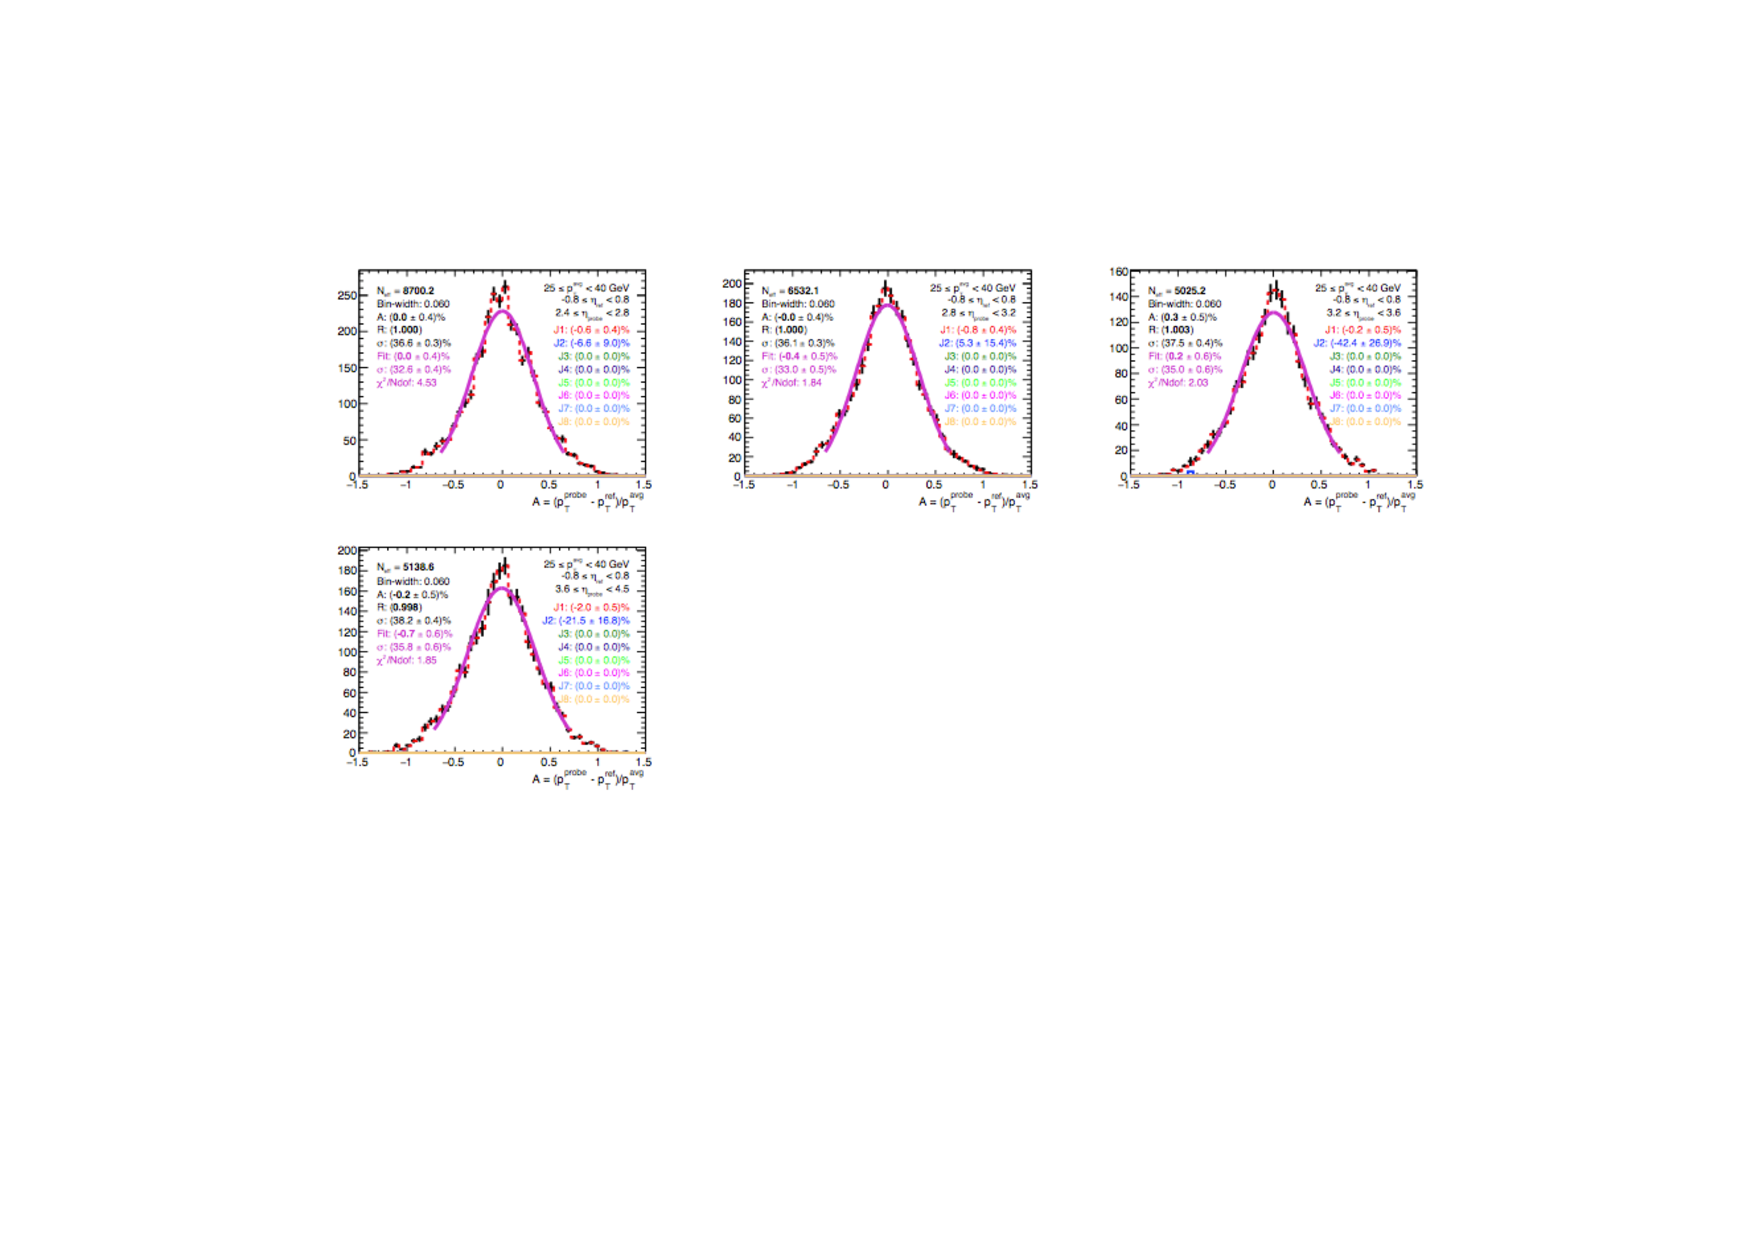
\includegraphics[width=9cm, height=5cm]{25to40PPTruthFits3.pdf}}
\end{frame}

\begin{frame}
\frametitle{Powheg+Pythia8 vs Sherpa}
\begin{columns}
\begin{column}{.4\textwidth}
\includegraphics[width=5cm, height=3.5cm]{25pTavg40_PowhegPythiavsSherpa.pdf}
\newline
\includegraphics[width=5cm, height=3.5cm]{55pTavg70_PowhegPythiavsSherpa.pdf}
\end{column}
\begin{column}{.4\textwidth}
\includegraphics[width=5cm, height=3.5cm]{85pTavg115_PowhegPythiavsSherpa.pdf}
\newline
\includegraphics[width=5cm, height=3.5cm]{145pTavg175_PowhegPythiavsSherpa.pdf}
\end{column}
\end{columns}
\end{frame}

\begin{frame}
\frametitle{Powheg+Pythia8 vs Sherpa: Problematic bins}
\begin{columns}
\begin{column}{.4\textwidth}
\includegraphics[width=4cm, height=3cm]{220pTavg270_PowhegPythiavsSherpa.pdf}
\newline
\includegraphics[width=4cm, height=3cm]{330pTavg400_PowhegPythiavsSherpa.pdf}
\end{column}
\begin{column}{.4\textwidth}
\includegraphics[width=4cm, height=3cm]{525pTavg760_PowhegPythiavsSherpa.pdf}
\newline
\includegraphics[width=4cm, height=3cm]{760pTavg1200_PowhegPythiavsSherpa.pdf}
\end{column}
\end{columns}
\begin{itemize}
\item The problems seem to lie in the extreme eta regions and so could be down to the definition of the resolution that I'm currently using.
\end{itemize}
\end{frame}

\begin{frame}
\frametitle{Powheg+Pythia8 subtraction}
\begin{columns}
\begin{column}{.3\textwidth}
\includegraphics[width=4.5cm, height=3cm]{Difference_PowhegPythia/55pTavg70_Difference.pdf}
\newline
\includegraphics[width=4.5cm, height=3cm]{Difference_PowhegPythia/70pTavg85_Difference.pdf}
\end{column}
\begin{column}{.4\textwidth}
\includegraphics[width=4.5cm, height=3cm]{Difference_PowhegPythia/85pTavg115_Difference.pdf}
\newline
\includegraphics[width=4.5cm, height=3cm]{Difference_PowhegPythia/115pTavg145_Difference.pdf}
\end{column}
\end{columns}
\begin{itemize}
\item Changed the resolution calculation to account for the EtaInterCal deviation from the run 1 method
\end{itemize}
\end{frame}

\begin{frame}
\frametitle{Sherpa subtraction...}
\begin{columns}
\begin{column}{.3\textwidth}
\includegraphics[width=4.5cm, height=3cm]{Difference_Sherpa/70pTavg85_Difference.pdf}
\newline
\includegraphics[width=4.5cm, height=3cm]{Difference_Sherpa/85pTavg115_Difference.pdf}
\end{column}
\begin{column}{.4\textwidth}
\includegraphics[width=4.5cm, height=3cm]{Difference_Sherpa/115pTavg145_Difference.pdf}
\newline
\includegraphics[width=4.5cm, height=3cm]{Difference_Sherpa/220pTavg270_Difference.pdf}
\end{column}
\end{columns}
\begin{itemize}
\item Lots of the points seem to be missing... any ideas?
\end{itemize}
\end{frame}

\begin{frame}
\frametitle{Calculating the resolution:}
\begin{itemize}
\item For jets in the same rapidity region: $\sigma$(A) = $\sqrt{2}$$\frac{\sigma(p_{T})}{p_{T}}$ 
\item If one of the two leading jets is in the probe region and the other is in the reference region: \newline \newline  $\frac{\sigma(p_{T})}{p_{T}}$ = $\sqrt{4\sigma^{2}(A_{(i,j)})-2\sigma^{2}(A_{(i,i)})}$ \newline
\item Need to correct for this
\end{itemize}
\end{frame}


\begin{frame}
\frametitle{To-do}
\begin{itemize}
\item Restrict the RMS value for the fits
\item Look into the missing points in the sherpa subtraction
\item Change the resolution definition to take into account the difference in asymmetry for the probe and reference rapidity regions
\end{itemize}
\end{frame}







\end{document} 